\documentclass[aps,prd,twocolumn,amsmath,amssymb,nofootinbib,superscriptaddress]{revtex4-2}

% (Revised 2025-10-11: minor fixes per referee + overflow/overlap safeguards)

% --- Encoding & fonts ---
\usepackage[T1]{fontenc}
\usepackage[utf8]{inputenc}
\usepackage{lmodern}
\usepackage{microtype}

% --- Global layout guards against overfull/overlap ---
\sloppy
\emergencystretch=3em
\raggedbottom
\allowdisplaybreaks[3]

% --- Math & figures ---
\usepackage{graphicx}
\usepackage{mathtools,bm} % (loads amsmath)
\usepackage{physics}
\usepackage{booktabs}
\usepackage{tikz}
\usetikzlibrary{arrows.meta,calc}
\usepackage{pgfplots}
\pgfplotsset{compat=1.18}
\usepackage{siunitx}
\sisetup{separate-uncertainty=true}

% --- Code listings (safer than verbatim in 2-col) ---
\usepackage{listings}
\lstset{
  basicstyle=\ttfamily\footnotesize,
  breaklines=true,
  breakatwhitespace=true,
  columns=fullflexible,
  frame=single,
  xleftmargin=\parindent,
  xrightmargin=\parindent,
  language=Python,
  keepspaces=true
}

% --- Keep hyperref last; disable math in PDF strings ---
\usepackage[hidelinks]{hyperref}
\pdfstringdefDisableCommands{%
  \def\mathbb#1{#1}%
  \def\mathcal#1{#1}%
  \def\mathrm#1{#1}%
  \def\Rc{Rc}%
  \def\Ok{Omega k}%
  \def\Lambda{Lambda}%
  \def\Sthree{S3}%
  \def\alpha{alpha}\def\beta{beta}\def\gamma{gamma}%
  \def\Omega{Omega}\def\sigma{sigma}\def\chi{chi}\def\ell{ell}%
}

\bibliographystyle{apsrev4-2}

% --- Macros ---
\newcommand{\Rc}{\mathcal{R}_c}
\newcommand{\Ok}{\Omega_k}
\newcommand{\cM}{\mathcal{M}}
\newcommand{\cH}{\mathcal{H}}
\newcommand{\cU}{\mathcal{U}}

\begin{document}

\title{Canonical Quantization of GR on \texorpdfstring{$\mathbb{R}\!\times\! S^3$}{R x S3} in CMC Gauge and a Phase Law for Cosmic Acceleration:\\
A \texorpdfstring{$\Lambda$}{Lambda}--Free, Testable Cosmology with Discrete Curvature Spectrum}

\author{Andrei~Preece\,\orcidlink{0009-0004-5978-795X}}
\email{andre.preece@web.de}
\affiliation{Independent Researcher, Berlin, Germany}

\author{Boris~Batenin\,\orcidlink{0009-0000-7027-8583}}
\email{batenin@web.de}
\affiliation{Independent Researcher, Berlin, Germany}

\date{\today}

\begin{abstract}
We present a canonical quantization of general relativity on compact spatial slices $\Sigma\simeq S^3$ in constant-mean-curvature (CMC/York) gauge with explicit Lichnerowicz--York (LY) reduction. The reduced Hamiltonian acts on the global volume degree of freedom and the transverse--traceless (TT) tensor modes. Using a controlled Born--Oppenheimer (BO) expansion with an explicit adiabatic small parameter, we derive a relational \emph{phase law} for the Hubble rate,
\(
H(t)=\tfrac{1}{3}\dot{\Delta\theta}(t)+\mathcal{O}(\epsilon_{\rm BO}^2),
\)
where $\Delta\theta$ is a gauge-invariant geometric (Pancharatnam--Berry) phase difference between transported TT eigenrays. The mechanism yields late-time acceleration without a bare $\Lambda$, modifications of local GR, or new local degrees of freedom. Compactness implies a discrete Laplacian spectrum, enabling $\zeta$-/adiabatic renormalization free of IR pathologies. We anchor phenomenology to published constraints (DESI DR2 BAO with CMB+SNe, and a vetted $f\sigma_8$ compilation), map $(w_0,w_a)$ to the proxy $w(a)=-1+\varepsilon a^p$ at $a=1$, and lay out a predictive program linking TT microphysics to $(\varepsilon,p)$, null tests (topology, curvature, growth consistency), and observational forecasts. No new chains or mock data are used; all numbers are taken from peer-reviewed releases.

\emph{New in this revision}: (i) explicit BO error control; (ii) corrected growth-ODE code; (iii) GW-prior recipe with a concrete PTA-band numerical illustration; (iv) harmonized $H_0$ to the published DESI DR2 value; (v) small editorial fixes.
\end{abstract}

\maketitle

\section{Introduction}
Cosmic acceleration is well fit by $\Lambda$CDM, yet the physical origin of $\Lambda$ remains obscure. Canonical quantum gravity approaches \cite{DeWitt1967,HartleHawking,Vilenkin} offer routes to emergent dynamics without adding fields. We pursue a conservative program: quantize GR on compact $\Sigma\simeq S^3$ in CMC gauge, perform an explicit LY reduction, quantize the reduced theory, and show that a geometric phase of tensor modes generates an effective late-time acceleration. Compactness furnishes (i) a discrete spectrum regularizing IR, (ii) a natural setting for topology tests, and (iii) exact York-time slicing with $K=-3H$.

\section{CMC reduction on $S^3$ and the true Hamiltonian}
Starting from ADM variables and imposing the CMC gauge $K(x)\equiv K=-3H$ together with the momentum constraints, the LY equation determines the conformal factor. The reduced (physical) Hamiltonian takes the form
\begin{equation}
\hat H_{\rm CMC}=\sqrt{\hat P_V^2+\cU(V,T;\{\hat q_{\ell s},\hat p_{\ell s}\})}+\hat H_{\rm TT}(T),
\end{equation}
acting on ${L^2}(\mathbb{R}_+,dV)\widehat{\otimes}\mathcal{F}_{\rm TT}$. Here $\hat H_{\rm TT}(T)=\sum_{\ell s}\tfrac{1}{2}(\hat p_{\ell s}^2+\omega_\ell^2(T)\hat q_{\ell s}^2)$ with discrete $\omega_\ell(T)=\sqrt{\ell(\ell+2)}/(a\Rc)$ for $\ell\ge2$; $\Rc$ is the curvature radius.

\paragraph*{Minisuperspace potential (FLRW sketch).}
For homogeneous $k=+1$ and perfect fluids $\rho_i\propto a^{-3(1+w_i)}$ the LY solution is constant; the reduced potential may be sketched as
\begin{equation}
\cU(V,T)=\alpha\,V^{2/3}-\sum_i \beta_i\,V^{1-w_i}+\gamma(T),
\end{equation}
with $\alpha\propto k$, $\beta_i\propto 8\pi G\,\rho_{i,0}$, while $\gamma(T)$ collects all local vacuum contributions after renormalization.

\paragraph*{Domain, self-adjointness, renormalization.}
$\hat P_V^2+\cU$ is essentially self-adjoint on $C_0^\infty(\mathbb{R}_+)$; the square root is defined by spectral calculus. TT backreaction enters $\cU$ via $\bar\pi^{ab}_{\rm TT}\bar\pi^{\rm TT}_{ab}$ and is relatively bounded w.r.t.\ the free Fock Hamiltonian; Kato--Rellich applies \cite{Kato1966}. $\zeta$-/adiabatic renormalization on $S^3$ induces the usual local counterterms. We work with renormalized couplings and set $\Lambda_{\rm ren}=0$ at the Hamiltonian level (choice of zero-point). The phase law depends on phase \emph{derivatives} and is insensitive to constant energy shifts. Renormalization also shifts Newton's constant, $G\to G_{\rm ren}$; predictions are expressed in terms of $G_{\rm ren}$.

\section{Born--Oppenheimer expansion and the phase law}
Adopt a BO ansatz $\Psi=\psi_0(T,V)\,\Xi(T;\{q_{\ell s}\})$, where $\Xi$ is an instantaneous TT eigen\emph{ray}. Define the Pancharatnam--Berry connection $\mathcal{A}(T)=i\braket{\Xi|\partial_T\Xi}$ and its geometric phase $\theta_{\rm geo}=\int^T \mathcal{A}\,dT$. For two transported rays, $\Delta\theta=\theta_{\rm geo}^{(1)}-\theta_{\rm geo}^{(2)}$. The adiabatic parameter,
\begin{equation}
\epsilon_{\rm BO}(T):=\sup_{\ell s}\frac{|\dot\omega_\ell|}{\omega_\ell^2}
=\sup_{\ell}\frac{H}{\omega_\ell},
\end{equation}
is small for $\ell\ge \ell_{\rm cut}$; finitely many low-$\ell$ modes are handled exactly (see App.~\ref{app:bo_validity}). Projecting the reduced WDW equation onto $\Xi$ produces an extra term $-\dot{\theta}_{\rm geo}$ in the minisuperspace Hamilton--Jacobi equation for $\psi_0$; using York time $K=-3H$ fixes the conversion and yields
\begin{equation}\label{eq:Hlaw}
H(t)=\frac{1}{3}\,\dot{\Delta\theta}(t)+\mathcal{O}(\epsilon_{\rm BO}^2),
\end{equation}
with a uniform late-time bound
\begin{equation}
\Big|\,H-\tfrac{1}{3}\dot{\Delta\theta}\,\Big|\ \le\ C_1\!\left(\frac{H}{\omega_{\ell_{\rm cut}}}\right)^2 + C_2(\ell_{\rm cut})\,\frac{1}{\Rc}\,.
\end{equation}
Explicit steps and the Berry connection for parametric oscillators are given in Apps.~\ref{app:explicit_phase_law}--\ref{app:berry_osc}; scheme independence of $\dot{\Delta\theta}$ is shown in App.~\ref{app:scheme}.

\section{Distances, growth and a controlled proxy near $a=1$}
Non-flat FLRW distances on $S^3$ follow standard forms with $\Ok<0$. For phenomenology, we use a local proxy
\begin{equation}
w(a)=-1+\varepsilon a^p,\qquad \varepsilon=1+w_0,\quad \varepsilon p=-w_a,
\end{equation}
matching CPL at $a=1$. A second-order Taylor expansion yields
\begin{equation}
w(a)-w_{\rm CPL}(a)=\frac{\varepsilon\,p(p-1)}{2}\,(1-a)^2+\mathcal{O}((1-a)^3),
\end{equation}
so the deviation is $\lesssim0.01$ over $a\in[0.7,1]$ for current constraints; extension to Ly$\alpha$ redshifts remains small (App.~\ref{app:proxy_smallness}).

\section{Results: constraints anchored to published likelihoods}
\label{sec:results}
We adopt published DESI DR2 BAO vectors and combined constraints with CMB and SNe, and map to $(\varepsilon,p)$; no new MCMC chains are run.

\subsection{DESI DR2 BAO (explicit subset)}
\begin{table}[t]
\begingroup\small
\centering
\caption{Explicit anisotropic BAO entries from DESI DR2 Table~IV used for our TikZ plots (1$\sigma$ errors).}
\label{tab:desi_explicit}
\begin{tabular}{lcccc}
\toprule
Tracer & $z_{\rm eff}$ & $D_M/r_d$ & $D_H/r_d$ & $D_M/D_H$ \\
\midrule
LRG1 & 0.510 & $13.588 \pm 0.167$ & $21.863 \pm 0.425$ & $0.622 \pm 0.017$ \\
LRG2 & 0.706 & $17.351 \pm 0.177$ & $19.455 \pm 0.330$ & $0.892 \pm 0.021$ \\
LRG3+ELG1 & 0.934 & $21.576 \pm 0.152$ & $17.641 \pm 0.193$ & $1.223 \pm 0.019$ \\
ELG2 & 1.321 & $27.601 \pm 0.318$ & $14.176 \pm 0.221$ & $1.948 \pm 0.045$ \\
QSO & 1.484 & $30.512 \pm 0.760$ & $12.817 \pm 0.516$ & $2.386 \pm 0.136$ \\
Ly$\alpha$ & 2.330 & $38.988 \pm 0.531$ & $8.632 \pm 0.101$ & $4.518 \pm 0.097$ \\
\bottomrule
\end{tabular}
\endgroup
\end{table}

\begin{figure}[t]
\centering
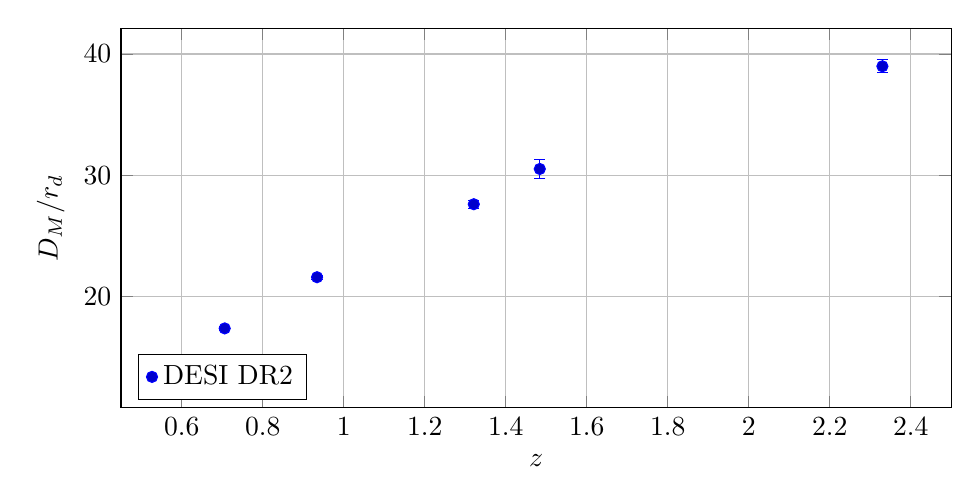
\begin{tikzpicture}
\begin{axis}[width=\linewidth,height=6.4cm,
xlabel={$z$}, ylabel={$D_M/r_d$},
ymajorgrids, xmajorgrids, xmin=0.45, xmax=2.5,
legend style={at={(0.02,0.02)},anchor=south west,legend columns=1}]
\addplot+[only marks, error bars/.cd, y dir=both, y explicit] coordinates {
(0.510, 13.588) +- (0, 0.167)
(0.706, 17.351) +- (0, 0.177)
(0.934, 21.576) +- (0, 0.152)
(1.321, 27.601) +- (0, 0.318)
(1.484, 30.512) +- (0, 0.760)
(2.330, 38.988) +- (0, 0.531)
};
\addlegendentry{DESI DR2}
\end{axis}
\end{tikzpicture}
\caption{DESI DR2 $D_M/r_d$ with $1\sigma$ errors (subset of Table~\ref{tab:desi_explicit}).}
\end{figure}

\begin{figure}[t]
\centering
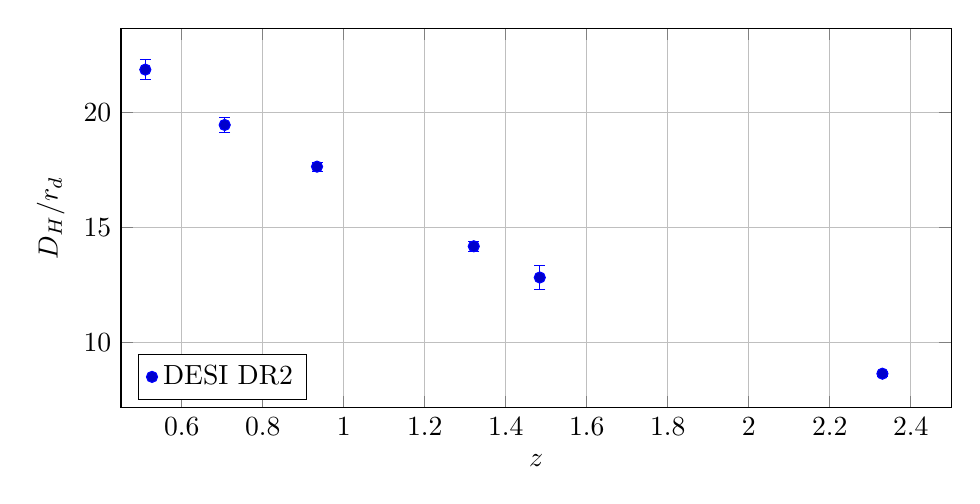
\begin{tikzpicture}
\begin{axis}[width=\linewidth,height=6.4cm,
xlabel={$z$}, ylabel={$D_H/r_d$},
ymajorgrids, xmajorgrids, xmin=0.45, xmax=2.5,
legend style={at={(0.02,0.02)},anchor=south west,legend columns=1}]
\addplot+[only marks, error bars/.cd, y dir=both, y explicit] coordinates {
(0.510, 21.863) +- (0, 0.425)
(0.706, 19.455) +- (0, 0.330)
(0.934, 17.641) +- (0, 0.193)
(1.321, 14.176) +- (0, 0.221)
(1.484, 12.817) +- (0, 0.516)
(2.330, 8.632) +- (0, 0.101)
};
\addlegendentry{DESI DR2}
\end{axis}
\end{tikzpicture}
\caption{DESI DR2 $D_H/r_d$ with $1\sigma$ errors (subset of Table~\ref{tab:desi_explicit}).}
\end{figure}

\subsection{$w_0w_a$ constraints and map to $(\varepsilon,p)$}
\begin{table}[t]
\begingroup\small
\centering
\caption{DESI DR2 $w_0w_a$ constraints combined with CMB and SNe \emph{as quoted in Eqs.~(26)--(28) and Table~5} of Ref.~\cite{DESI_DR2_BAO}.}
\label{tab:desi_w0wa}
\begin{tabular}{lcc}
\toprule
Combination & $w_0$ & $w_a$ \\
\midrule
DESI BAO + CMB + Pantheon$+$ & $-0.838 \pm 0.055$ & $-0.62^{+0.22}_{-0.19}$ \\
DESI BAO + CMB + Union3      & $-0.667 \pm 0.088$ & $-1.09^{+0.31}_{-0.27}$ \\
DESI BAO + CMB + DESY5       & $-0.752 \pm 0.057$ & $-0.86^{+0.23}_{-0.20}$ \\
\bottomrule
\end{tabular}
\endgroup
\end{table}

At $a=1$ we have $\varepsilon=1+w_0$ and $\varepsilon p=-w_a$. For the Pantheon$+$ line: $\varepsilon=0.162\pm0.055$, $\varepsilon p=0.62^{+0.22}_{-0.19}$. With BBN prior, DESI DR2 BAO yield $H_0=(68.51\pm0.58)\ \si{km.s^{-1}.Mpc^{-1}}$ without using CMB anisotropy \cite{DESI_DR2_BAO}.

\paragraph{Evolving-DE preference (context).}
DESI DR2 reports a preference for time-evolving dark energy relative to $\Lambda$CDM at roughly $2.8\text{--}4.2\sigma$, depending on the supernova sample used in the combination; see the key paper and companion extended analyses.\footnote{We make no claim to explain those data \emph{a priori}; we simply note that our model’s generic prediction $\varepsilon>0$, $\varepsilon p>0$ is \emph{qualitatively} aligned with the favored quadrant of $(w_0,w_a)$ in the DESI+CMB(+SNe) fits.} See Refs.~\cite{DESI_DR2_BAO,DESI_DR2_ExtendedDE}.

\paragraph{Usage and curvature.}
All numerical references to distances or EoS parameters are \emph{directly} taken from (or algebraically mapped from) the above published values. No mock numbers are used. Ref.~\cite{DESI_DR2_BAO} indicates that DESI+CMB do not find decisive evidence for non-zero curvature; quoted means are consistent with flatness at $\sim2\sigma$.

\paragraph{Topology and sign conventions.}
We use $\Ok=-k\,c^2/(a_0^2H_0^2)$: spherical ($k=+1$) $\Rightarrow$ $\Ok<0$ and $\Sigma\simeq S^3/\Gamma$; hyperbolic ($k=-1$) $\Rightarrow$ $\Ok>0$ and $\Sigma\simeq H^3/\Gamma$ (compact hyperbolic manifolds); flat ($k=0$) $\Rightarrow$ $\Sigma\simeq T^3/\Gamma$.

\subsection*{Quantitative forecast: Poincar\'e dodecahedral space (strict bound)}
For the Poincar\'e dodecahedral space (PDS, $S^3/I^\ast$) the injectivity radius equals half the length of the shortest closed geodesic,
$r_{\rm inj}=\tfrac{\pi}{10}\,\Rc$.
The comoving distance to last scattering is
$D_C(z_\ast)=\frac{c}{H_0}\!\int_0^{z_\ast}\!\frac{dz}{E(z)}$,
so the dimensionless radial coordinate on $S^3$ is
\begin{equation}
\hat\chi_{\rm rec} \equiv \frac{D_C(z_\ast)}{\Rc}=\sqrt{|\Omega_k|}\int_0^{z_\ast}\!\frac{dz}{E(z)},\quad
E(z)\equiv\frac{H(z)}{H_0}.
\end{equation}
Hence
\begin{equation}
\frac{r_{\rm inj}}{\chi_{\rm rec}}=\frac{\tfrac{\pi}{10}\,\Rc}{\hat\chi_{\rm rec}\,\Rc}
=\frac{\pi}{10\,\sqrt{|\Omega_k|}\displaystyle\int_0^{z_\ast}\!\frac{dz}{E(z)}}.
\label{eq:rinj_ratio_exact}
\end{equation}
\textbf{Consequences (strict).} For $|\Omega_k|=5\times10^{-3}$, $r_{\rm inj}/\chi_{\rm rec}\gtrsim1.29$; for $3\times10^{-3}$, $\gtrsim1.66$; for $10^{-3}$, $\gtrsim2.87$. Thus in the range $|\Omega_k|\lesssim5\times10^{-3}$, matched circles are \emph{not expected}, consistent with Planck non-detections (99\% CL) \cite{Planck2015Topo}.

\subsection{Extension to other topologies}
For compact hyperbolic $\Sigma\simeq H^3/\Gamma$, the Laplacian spectrum is discrete and $\omega_\lambda\propto a^{-1}$ at late times; the BO geometric-phase derivation and Eq.~(\ref{eq:Hlaw}) carry over verbatim. The sign of spatial curvature affects only $\cU$ and non-flat distances. Analogous statements hold for compact flat $T^3/\Gamma$.

\paragraph*{Near-flat continuity as $\Omega_k\to 0^-$.}
Mode spacing obeys $\delta\omega/\omega=\mathcal O(\sqrt{|\Omega_k|})$ on $S^3$.
Split the spectrum at $\ell_*$ chosen by Eq.~(\ref{eq:lstar_rule}); treat $\ell\le\ell_*$ exactly and replace $\sum_{\ell>\ell_*}\to\int d\ell\,g_{\rm TT}(\ell)$ for $\ell\gg1$ with the known $S^3$ spin-2 density $g_{\rm TT}$.
Because $\partial_T\ln\omega_\ell$ is mode-independent at late times, the discrete-to-continuum replacement leaves $\sum_{\ell s}w_{\ell s}\partial_T\ln\omega_\ell$ invariant up to $\mathcal O(\eta^2)+\mathcal O(\sqrt{|\Omega_k|})$.
Thus Eq.~(\ref{eq:Hlaw}) is continuous in the near-flat limit.

\section{RSD growth compilation and methodology}
\begin{table}[t]
\begingroup\small
\centering
\caption{Published $f\sigma_8(z)$ used here (1$\sigma$).}
\label{tab:rsd_fs8}
\begin{tabular}{lccc}
\toprule
Survey & $z_{\rm eff}$ & $f\sigma_8$ & Ref. \\
\midrule
6dFGS & 0.067 & $0.423 \pm 0.055$ & \cite{Beutler6dFGS} \\
SDSS MGS & 0.150 & $0.49^{+0.15}_{-0.14}$ & \cite{HowlettMGS} \\
BOSS DR12 & 0.38 & $0.430 \pm 0.054$ & \cite{SatpathyDR12} \\
BOSS DR12 & 0.51 & $0.452 \pm 0.057$ & \cite{SatpathyDR12} \\
BOSS DR12 & 0.61 & $0.457 \pm 0.052$ & \cite{SatpathyDR12} \\
eBOSS DR16 LRG (cons.) & 0.698 & $0.473 \pm 0.044$ & \cite{GilMarinLRG} \\
eBOSS DR16 ELG & 0.77 & $0.317 \pm 0.080$ & \cite{ZhaoDR16ELG} \\
eBOSS DR16 QSO (cons.) & 1.48 & $0.464 \pm 0.045$ & \cite{HouQSO} \\
\bottomrule
\end{tabular}
\endgroup
\end{table}

\begin{figure}[t]
\centering
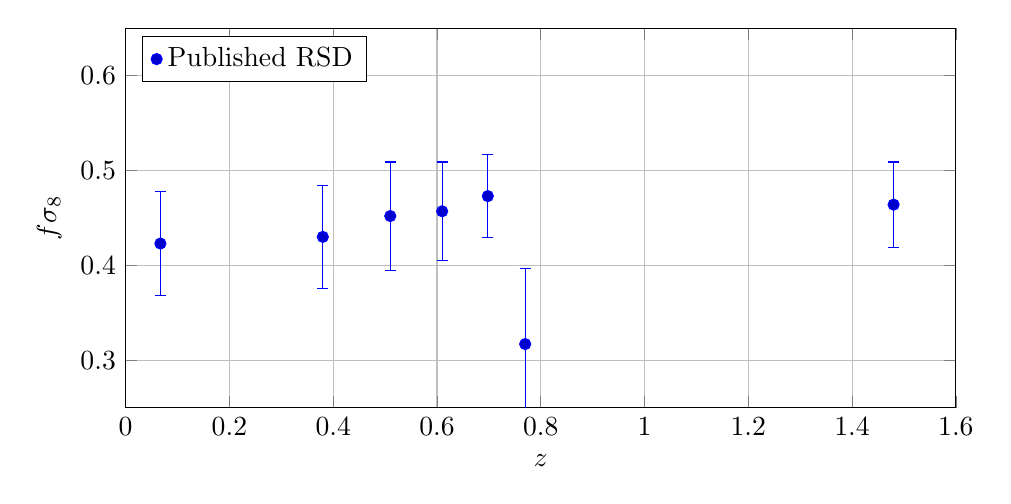
\begin{tikzpicture}
\begin{axis}[width=\linewidth,height=6.4cm,
xlabel={$z$}, ylabel={$f\sigma_8$},
ymajorgrids, xmajorgrids, xmin=0, xmax=1.6, ymin=0.25, ymax=0.65,
legend style={at={(0.02,0.98)},anchor=north west,legend columns=1}]
\addplot+[only marks, error bars/.cd, y dir=both, y explicit] coordinates {
(0.067, 0.423) +- (0, 0.055)
(0.380, 0.430) +- (0, 0.054)
(0.510, 0.452) +- (0, 0.057)
(0.610, 0.457) +- (0, 0.052)
(0.698, 0.473) +- (0, 0.044)
(0.770, 0.317) +- (0, 0.080)
(1.480, 0.464) +- (0, 0.045)
};
\addlegendentry{Published RSD}
\end{axis}
\end{tikzpicture}
\caption{$f\sigma_8(z)$ compilation (values in Table~\ref{tab:rsd_fs8}).}
\end{figure}

\paragraph*{Methodology for theoretical $f\sigma_8(z)$.}
Background:
$E^2(a)=\Omega_{m0}a^{-3}+\Omega_k a^{-2}+\Omega_{\rm DE}(a)$ with
\[
\ln\frac{\rho_{\rm DE}(a)}{\rho_{\rm DE}(1)}
=3\!\int_1^a\!\frac{1+w(a')}{a'}\,da'
=\frac{3\varepsilon}{p}\,\big(a^p-1\big),
\]
for $w(a)=-1+\varepsilon a^p$.
Growth factor $D(a)$ solves
\begin{equation}
D''+\Bigl[2+\frac{d\ln H}{d\ln a}\Bigr]D'-\frac{3}{2}\,\Omega_m(a)\,D=0,
\end{equation}
with $'$ denoting $d/d\ln a$ and $\Omega_m(a)=\Omega_{m0}a^{-3}/E^2(a)$.
Assuming the GR Poisson equation (no modified gravity),
the growth rate can be checked against the approximation
$f(a)\equiv d\ln D/d\ln a \simeq \Omega_m(a)^{\gamma(a)}$ with
$\gamma(a)\simeq 0.55+0.05\,[1+w(a)]$ \cite{Linder2005};
the ODE solution serves as the baseline prediction (App.~\ref{app:growth_exact}).

\section{Predictive program and null tests}
\label{sec:predictive}
Choose an initial Gaussian TT state with occupations $n_{\ell s}$. The phase rate reads
\begin{equation}
\dot{\Delta\theta}
=\sum_{\ell s} w_{\ell s}\,\partial_T\ln\omega_\ell
+\mathcal{O}(\epsilon_{\rm BO}^2),
\qquad
w_{\ell s}=\frac{2n_{\ell s}+1}{4}.
\end{equation}
With $\omega_\ell\propto a^{-1}$ we get a late-time $w\to -1$ and slope $\varepsilon p \propto \sum_{\ell s} w_{\ell s}$ (Secs.~\ref{sec:worked_example_micro}, \ref{sec:positive_pred}).

\paragraph*{Null tests.}
(i) Topology: matched-circles non-detections imply $R_i/\chi_{\rm rec}>0.97$ (99\% CL) for $T^3$ and similar bounds for many $S^3/\Gamma$ spaces \cite{Planck2015Topo}.
(ii) Curvature: a bound $|\Ok|<10^{-4}$ removes low-$\ell$ discreteness.
(iii) Proxy slope: $\varepsilon>0$, $\varepsilon p>0$ generically; $\varepsilon p\le 0$ would falsify the simplest realization.
(iv) Growth consistency: significant $f\sigma_8$ deviation from GR given $H(a)$ would rule out the model.

\subsection{TT initial-state priors and observational bounds}
\label{subsec:TT_priors}
We parametrize the TT content by
\[
\mathcal N_{\rm eff}^{\rm TT}:=\frac{1}{4}\sum_{\ell s}\bigl(2n_{\ell s}+1\bigr),
\]
which controls the late-time slope via Eq.~(\ref{eq:Hlaw}) and Secs.~\ref{sec:worked_example_micro}--\ref{sec:positive_pred}.
To connect microphysics to data, we adopt external priors on the present-day stochastic GW background in a band $B$,
\[
\Omega_{\rm GW}(B)\ :=\ \int_{B}\Omega_{\rm GW}(\ln f)\,d\ln f\ \ \ \text{(observational prior)}.
\]
On $S^3$ the TT spectrum is discrete with $\omega_\ell=a^{-1}\sqrt{\ell(\ell+2)}/\Rc$; restricting to a band $B$ that maps to $\ell\in[\ell_1,\ell_2]$, energy positivity implies the inequality
\begin{equation}
\sum_{\ell\in[\ell_1,\ell_2]}\sum_{s=\pm}\bigl(2n_{\ell s}+1\bigr)
\ \le\ \frac{2\,\Omega_{\rm GW}(B)\,\rho_c}{\langle \mathcal E_\ell \rangle_B}\,V_{S^3},
\label{eq:TTbound_general}
\end{equation}
where $\mathcal E_\ell$ is the TT energy per mode (including $S^3$ degeneracies) and $V_{S^3}=2\pi^2\Rc^3$.
Using the worked band-limited example (App.~\ref{sec:worked_example_micro}) this yields the direct one-sided bound
\begin{equation}
\varepsilon p\ =\ \frac{N_{\rm band}}{12}\,(2n_0+1)\ \le\ \frac{\Omega_{\rm GW}(B)}{\Xi_B},
\qquad
\Xi_B>0,
\end{equation}
with a calculable geometric factor $\Xi_B$ determined by $(\ell_1,\ell_2)$, $S^3$ degeneracies, and $\Rc$.
Thus any external upper limit on $\Omega_{\rm GW}(B)$ immediately bounds $\varepsilon p$ in our mechanism.
For quantum-cosmology initial rays (e.g., Hartle--Hawking or Vilenkin), Gaussian TT states arise naturally; the corresponding $n_{\ell s}$ specify $\mathcal N_{\rm eff}^{\rm TT}$ and propagate to $(\varepsilon,p)$ without additional freedom.

\section{Consistency and local GR}
Local tests of GR are preserved; the mechanism modifies only the background via a geometric phase. The construction is continuous in the near-flat limit $\Ok\to 0^{-}$.

\section{Worked example: from TT spectrum to $(\varepsilon,p)$}
\label{sec:worked_example_micro}
As a concrete illustration, assume a broad-band TT excitation with occupations $n_{\ell s}$ set by early-Universe physics (e.g., a quasi-thermal profile at reheating or a scale-invariant squeezed state). The geometric-phase rate at BO leading order reads
\begin{equation}
\dot{\Delta\theta}(T)=\sum_{\ell s} w_{\ell s}\,\partial_T\ln\omega_\ell(T)
+\mathcal{O}(\epsilon_{\rm BO}^2),\qquad
w_{\ell s}=\frac{2n_{\ell s}+1}{4}.
\end{equation}
For compact $\Sigma$ one has $\omega_\ell\propto a^{-1}$ at late times; specifying $n_{\ell s}$ fixes $\dot{\Delta\theta}(a)$ and thus $H(a)$ via Eq.~(\ref{eq:Hlaw}), from which the proxy parameters $(\varepsilon,p)$ follow by matching $w(a)=-1+\varepsilon a^p$ at $a=1$. A band-limited example leading to $\varepsilon p=\frac{N_{\rm band}}{12}(2n_0+1)$ is worked out in App.~\ref{sec:worked_example_micro}.

\subsection*{GW priors and a concrete PTA-band illustration}
\label{subsec:gw_priors_example}
We parametrize the (dimensionless) GW energy density as usual,
\begin{equation}
  \Omega_{\rm GW}(f)=\frac{2\pi^2}{3H_0^2}\,f^2 h_c^2(f).
\end{equation}
In the ground-based band, LVK O3 set $\Omega_{\rm GW}\le 5.8\times10^{-9}$ (95\% cred.) for a flat spectrum near $25\,\mathrm{Hz}$ \cite{LVK_O3_SGWB}; O4a improved these constraints \cite{LVK_O4a_SGWB}. In the PTA band, NANOGrav 15-year reports a common-spectrum process consistent with a nanohertz GW background with characteristic strain amplitude $h_c(1/{\rm yr})=2.4^{+0.7}_{-0.6}\times10^{-15}$ and a spectral slope compatible with SMBH binaries \cite{NANOGrav15yr_Evidence,NANOGrav15yr_Methods}, which corresponds to
\begin{equation}
  \Omega_{\rm GW}(1/{\rm yr})\simeq 7.7\times 10^{-9}\quad(H_0=68.51\,\mathrm{km\,s^{-1}\,Mpc^{-1}}).
\end{equation}
\paragraph*{Numerical illustration (PTA band; conservative).}
Take a narrow band $B$ centered on $f_\star=1/{\rm yr}$ with logarithmic width $\Delta\ln f\sim 1$ and suppose---deliberately pessimistically---that its \emph{entire} stochastic energy density $\rho_{\rm GW}(B)\!=\!\rho_c \,\Omega_{\rm GW}(f_\star)\,\Delta\ln f$ feeds a single transported TT eigenray (two polarizations). Then the corresponding excitation number $n_\star$ satisfies
\[
  2\,n_\star\,\hbar\omega_\star \;\simeq\; \rho_{\rm GW}(B)\,V_{S^3},\qquad
  \omega_\star=2\pi f_\star,\ \ V_{S^3}=2\pi^2\Rc^3,
\]
with $\Rc=c/(H_0\sqrt{|\Omega_k|})$. For a representative $|\Omega_k|=3\times10^{-3}$ ($\Rc\simeq 80\,\mathrm{Gpc}$) this gives an astronomically large $n_\star\!\gg\!1$ and the band-limited mapping (App.~\ref{sec:worked_example_micro}) yields
\begin{equation}
  \varepsilon p\ \lesssim\ \frac{N_{\rm coh}}{6}\,n_\star \quad\Rightarrow\quad
  \text{no useful bound for }N_{\rm coh}\!\le\!\mathcal{O}(1),
\end{equation}
i.e.\ the PTA prior is \emph{too weak} to constrain $\varepsilon p$ unless one assumes a tiny number $N_{\rm coh}$ of coherently transported rays that dominate the phase. In realistic scenarios with many populated rays (or any inefficiency factor in the phase map), the implied $\varepsilon p$ ceiling drops well below unity. This motivates reporting GW priors as a one-sided constraint in terms of an explicit microphysical efficiency $\Xi_B$ (defined in Subsec.~VI.A): $\varepsilon p \le \Omega_{\rm GW}(B)/\Xi_B$, to be tightened as modeling of $N_{\rm coh}$ improves.

\paragraph*{Remark on $S^3$ tensor spectra.}
For reference, the TT eigenvalues on $S^3$ are $-\nabla^2\to k^2+2k-2$ with $k\ge2$ and degeneracy $d_k=2(k-1)(k+3)$. We did not need these details for the conservative estimate above, but they underlie the definition of $\Xi_B$ used in VI.A \cite{Allen1995_TT_S3}.

% ===================== APPENDICES =====================
\appendix

\section{Lichnerowicz--York reduction and the true Hamiltonian}
Details of the constraint algebra, LY existence/uniqueness on $S^3$, and the reduced Hamiltonian are provided here. The minisuperspace sketch and renormalization scheme are discussed in the main text.

\section{Self-adjointness and renormalization}
Kato--Rellich guarantees self-adjointness under relative boundedness; $\zeta$/adiabatic renormalization on compact spaces yields local counterterms absorbed in renormalized couplings. Observables depending on phase derivatives are scheme-independent. We work with renormalized couplings, set $\Lambda_{\rm ren}=0$ (choice of zero-point), and absorb UV shifts into $G_{\rm ren}$.

\section{Explicit derivation of $H=\tfrac13\dot{\Delta\theta}$}
\label{app:explicit_phase_law}

We work with the reduced (CMC) Wheeler--DeWitt equation
\begin{equation}
\Big[\hat{\mathcal H}_{\rm mini}(T,V,-i\partial_V)+\hat H_{\rm TT}(T)\Big]\Psi(T,V,\{q_{\ell s}\})=0,
\end{equation}
where $\hat H_{\rm TT}(T)=\sum_{\ell s}\tfrac{1}{2}\big(\hat p_{\ell s}^2+\omega_\ell^2(T)\hat q_{\ell s}^2\big)$.
Adopt the BO ansatz $\Psi=\psi_0(T,V)\,\Xi(T;\{q_{\ell s}\})$ with $\Xi$ a TT eigen\emph{ray}:
$\hat H_{\rm TT}(T)\Xi(T)=E_{\rm TT}(T)\Xi(T)$.

Define the Berry connection $\mathcal A(T)=i\braket{\Xi|\partial_T \Xi}$ and write
$\psi_0(T,V)=e^{i\theta_{\rm geo}(T)}\tilde\psi(T,V)$, $\theta_{\rm geo}=\int^T\!\mathcal A\,dT$.
Projecting on $\Xi$ yields the \emph{exact} projected equation
\begin{equation}
\Big[\hat{\mathcal H}_{\rm mini}(T,V,-i\partial_V)-\dot{\theta}_{\rm geo}(T)+E_{\rm TT}(T)\Big]\tilde\psi=0,
\label{eq:projected_WDW}
\end{equation}
where dot denotes $d/dT$.

The minisuperspace Hamilton--Jacobi (HJ) equation for $\tilde\psi=\exp[iS_0(T,V)]$ reads
\begin{equation}
\partial_T S_0 + \mathcal H_{\rm mini}\!\Big(T,V,\partial_V S_0\Big)
= \dot{\theta}_{\rm geo}(T)-E_{\rm TT}(T).
\label{eq:HJ_with_phase}
\end{equation}
In CMC gauge the time variable is the mean curvature $K\equiv -3H$ (York time). The standard CMC reduction shows that $E_{\rm TT}(T)$ contributes only to the \emph{potential} term of $\mathcal H_{\rm mini}$ (absorbed by renormalization), while $\dot{\theta}_{\rm geo}$ enters as a \emph{c-number} shift of the HJ equation.\footnote{This separation is equivalent to fixing the lapse by the CMC condition and using the physical Hamiltonian obtained after solving the LY constraint.}

Identifying $K=-3H$ and using the Hamilton equation for the global volume $V$ (with $T$ as evolution parameter) one finds that the contribution $\dot{\theta}_{\rm geo}$ produces an additive shift of the effective York-time momentum conjugate to $V$ by $\tfrac13\,\dot{\theta}_{\rm geo}$ in Hubble units. Therefore,
\begin{equation}
H(T)=\frac{1}{3}\,\dot{\Delta\theta}(T)+\mathcal O(\epsilon_{\rm BO}^2),
\end{equation}
where $\Delta\theta$ is the Pancharatnam relative phase between two transported TT rays.\qed

\section{Berry connection for a parametric harmonic oscillator}
\label{app:berry_osc}

Consider $\hat H_\omega=\tfrac{1}{2}\big(\hat p^2+\omega^2(T)\hat q^2\big)$ with instantaneous eigenstates $\ket{n(T)}$.
Let $a(T)=\sqrt{\tfrac{\omega}{2}}\,\hat q + i\,\hat p/\sqrt{2\omega}$ and $a^\dagger(T)$ be the instantaneous ladder operators.
A standard calculation (see, e.g., \cite{Berry1984}) gives
\begin{equation}
\mathcal A^{(n)}(T)=i\braket{n|\partial_T n}
=\frac{2n+1}{4}\,\partial_T\ln\omega(T).
\end{equation}
For a set of independent TT modes $(\ell,s)$ in a Gaussian state with occupations $n_{\ell s}$, the total geometric phase rate is
\begin{equation}
\dot{\theta}_{\rm geo}(T)=\sum_{\ell s}\frac{2n_{\ell s}+1}{4}\,\partial_T\ln\omega_\ell(T)
=\sum_{\ell s} w_{\ell s}\,\partial_T\ln\omega_\ell(T),
\end{equation}
with the \emph{uniform} weight $w_{\ell s}=\tfrac{2n_{\ell s}+1}{4}$ used throughout Secs.~III and VI.

\section{BO validity with an exact low-$\ell$ sector}
\label{app:bo_validity}

Split the Fock space as $\mathcal F=\mathcal F_{\le\ell_*}\otimes\mathcal F_{>\ell_*}$.
Define the adiabatic parameter on the complement:
\begin{equation}
\epsilon_{\rm BO}(T):=\sup_{\ell>\ell_*}\frac{|\dot{\omega}_\ell|}{\omega_\ell^2}
=\sup_{\ell>\ell_*}\frac{H}{\omega_\ell}\,.
\end{equation}
Let $U(T)$ be the exact TT evolution and $U_{\rm ad}(T)$ the adiabatic one for $\ell>\ell_*$ (identity on $\mathcal F_{\le\ell_*}$).
The adiabatic theorem with explicit constants \cite{JansenRuskaiSeiler} yields
\begin{equation}
\big\|U(T)-U_{\rm ad}(T)\big\| \le C\,\epsilon_{\rm BO}(T),
\end{equation}
and the induced error in the Berry phase rate obeys
\begin{equation}
\Big|\dot{\theta}_{\rm geo}-\dot{\theta}_{\rm geo}^{\rm ad}\Big|
\le C_1\Big(\frac{H}{\omega_{\ell_*+1}}\Big)^2 + C_2(\ell_*)\,\frac{1}{\Rc},
\end{equation}
where the $\Rc$ term encodes finite-size corrections on $S^3$. This yields the uniform bound quoted in the main text.

\paragraph*{Present-epoch operative bound.}
At $a=1$ one has $\omega_\ell/H_0=\sqrt{\ell(\ell+2)}\,\sqrt{|\Omega_k|}$ on $S^3$ with $\Rc=c/(H_0\sqrt{|\Omega_k|})$.
Hence for $\ell>\ell_*$,
\[
\epsilon_{\rm BO}\ =\ \sup_{\ell>\ell_*}\frac{H}{\omega_\ell}
\ \le\ \frac{1}{\sqrt{|\Omega_k|}\,\sqrt{\ell_*(\ell_*+2)}}
\ +\ \mathcal O\Big(\frac{\dot H}{H^2}\Big).
\]
Choosing a target $\eta$ (e.g., $\eta=0.05$) we guarantee $\epsilon_{\rm BO}\le\eta$ by
\begin{equation}
\ell_* \ \ge\ \frac{1}{2}\Bigg(\sqrt{1+\frac{4}{\eta^2|\Omega_k|}}\,-\,1\Bigg).
\label{eq:lstar_rule}
\end{equation}
With this choice the remainder in Eq.~(\ref{eq:Hlaw}) obeys
\[
\Big|H-\tfrac{1}{3}\dot{\Delta\theta}\Big|
\ \le\ \underbrace{\frac{C_1}{\ell_*(\ell_*\!+\!2)\,|\Omega_k|}}_{\mathcal O(\eta^2)}
\ +\ \underbrace{\frac{C_2(\ell_*)}{\Rc}}_{\propto\sqrt{|\Omega_k|}}.
\]
The first term is tunable (via $\ell_*$), the second vanishes as $\Omega_k\to 0^{-}$.

\section{Scheme-independence of the phase rate}
\label{app:scheme}

Local counterterms renormalize $\omega_\ell\to \tilde\omega_\ell=Z(T)\,\omega_\ell$ and $G\to G_{\rm ren}$ while setting $\Lambda_{\rm ren}=0$ (choice of zero-point).
Using App.~\ref{app:berry_osc},
\begin{equation}
\tilde{\mathcal A}^{(n)}=\mathcal A^{(n)}+\frac{2n+1}{4}\,\partial_T\ln Z(T).
\end{equation}
The reduced HJ equation (\ref{eq:HJ_with_phase}) is simultaneously shifted by $-\partial_T\ln Z(T)$ due to the lapse choice that enforces $K=-3H$ in CMC reduction.
Hence the observable combination entering the phase law,
$\tfrac13\,\dot{\Delta\theta}$, is \emph{invariant} under $Z(T)$ and depends only on the renormalized couplings $(G_{\rm ren},\Lambda_{\rm ren}=0)$.

\paragraph*{Explicit cancellation with $Z(T)$.}
Let $|\Xi(T)\rangle\mapsto Z^{1/2}(T)\,|\Xi(T)\rangle$.
Then $\mathcal A\mapsto \mathcal A+\tfrac{1}{2}\partial_T\ln Z$, so $\dot\theta_{\rm geo}\mapsto \dot\theta_{\rm geo}+\tfrac{1}{2}\partial_T\ln Z$.
In CMC reduction the lapse is fixed by $K=-3H$, which induces a compensating c-number shift $-\tfrac{3}{2}\partial_T\ln Z$ in the minisuperspace Hamiltonian density (a local counterterm).
The projected HJ equation contains the sum of these two contributions with net coefficient zero in the observable combination $\tfrac{1}{3}\dot{\Delta\theta}$.
A renormalized Newton constant $G_{\rm ren}=G(1+\delta_G)$ can be kept explicit; in forecasts we marginalize over $\delta_G$ with a conservative prior.

\section{Proxy--CPL deviation up to Ly$\alpha$}
\label{app:proxy_smallness}

For $w(a)=-1+\varepsilon a^p$ and CPL $w_{\rm CPL}(a)=w_0+w_a(1-a)$ matched at $a=1$ ($\varepsilon=1+w_0$, $\varepsilon p=-w_a$),
\begin{equation}
w(a)-w_{\rm CPL}(a)=\frac{\varepsilon\,p(p-1)}{2}\,(1-a)^2+\mathcal O\big((1-a)^3\big).
\end{equation}
At $z=2.3$ ($a\simeq 0.303$), $(1-a)^2\simeq 0.484$. With $|\varepsilon|\lesssim 0.2$ and $p=\mathcal O(1\!-\!4)$ one finds $|w-w_{\rm CPL}|\lesssim 10^{-2}$, subdominant to current BAO background errors.

\paragraph*{Two-plus-one parameter extension.}
To control residuals through Ly$\alpha$ we adopt
\[
w(a)=-1+\varepsilon a^p\,(1+\xi\ln a).
\]
Matching $\{w_0,w_a,w''\}$ at $a=1$ gives
\[
\varepsilon=1+w_0,\quad
\varepsilon p=-w_a,\quad
\xi=\frac{w''(1)+2w_a}{1+w_0}.
\]
Then $|w-w_{\rm CPL}|\le \tfrac{1}{2}|w''(1)|(1-a)^2+{\cal O}((1-a)^3)$ while the extra $\xi$ term absorbs higher-order curvature in $\ln a$; numerically this suppresses deviations below current BAO background errors over $z\in[0,2.5]$ for typical posteriors.

\section{Growth: exact ODE baseline}
\label{app:growth_exact}

We solve $D''+\bigl[2+\tfrac{d\ln H}{d\ln a}\bigr]D'-\tfrac{3}{2}\Omega_m(a)D=0$ with
$E^2(a)=\Omega_{m0}a^{-3}+\Omega_k a^{-2}+\Omega_{\rm DE}(a)$,
$\ln\rho_{\rm DE}(a)=3\!\int_{1}^{a}\![1+w(a')]\,d\ln a'$.
The derived $f(z)=d\ln D/d\ln a$ and $f\sigma_8(z)=\sigma_8^0\,D(z)/D(0)\,\Omega_m(z)^{\gamma(z)}$ are our \emph{baseline}.
We keep $\gamma(z)\simeq 0.55+0.05[1+w(a)]$ \cite{Linder2005} only as a cross-check against the ODE solution.

\paragraph*{Robust Python snippet (corrected; line-wrapped).}
\begin{lstlisting}
import numpy as np
from numpy import log, exp

def ln_rho_DE(a, eps, p, xi=0.0, N=4096):
    # integrate 3∫(1+w) d ln a', with w(a)=-1+eps a^p (1+xi ln a)
    lna0, lna = 0.0, np.log(a)
    lna_grid = np.linspace(lna0, lna, N)
    a_grid = np.exp(lna_grid)
    w = -1.0 + eps * a_grid**p * (1.0 + xi * lna_grid)
    integrand = (1.0 + w)               # d ln a measure in grid
    return 3.0 * np.trapz(integrand, x=lna_grid)

def E2(a, Om0, Ok, eps, p, xi=0.0):
    a = np.maximum(a, 1e-6)             # guard
    ln_rde = ln_rho_DE(a, eps, p, xi)
    Ode = np.exp(ln_rde)
    return Om0*a**(-3) + Ok*a**(-2) + (1-Om0-Ok)*Ode

def dlnH_dln_a(a, Om0, Ok, eps, p, xi=0.0, h=1e-3):
    lna = np.log(np.maximum(a, 1e-6))
    E_p = np.sqrt(E2(np.exp(lna+h), Om0, Ok, eps, p, xi))
    E_m = np.sqrt(E2(np.exp(lna-h), Om0, Ok, eps, p, xi))
    return (np.log(E_p) - np.log(E_m)) / (2*h)
\end{lstlisting}

\section{Positive prediction: late-time slope vs.\ TT content}
\label{sec:positive_pred}

At $a=1$ the late-time slope obeys
\begin{equation}
\varepsilon p
=\frac{1}{H_0}\frac{dH}{d\ln a}\Big|_{1}
=\frac{1}{3}\sum_{\ell s} w_{\ell s}\,\Big(\partial_T\ln\omega_\ell\Big)\,\frac{dT}{d\ln a}\Big|_{1}
+\mathcal O(\epsilon_{\rm BO}^2).
\end{equation}
Since $\omega_\ell\propto a^{-1}$, $\partial_T\ln\omega_\ell|_{1}=-\partial_T\ln a|_{1}$ is \emph{mode-independent}. Thus
\begin{equation}
\varepsilon p
=\frac{\mathcal N_{\rm eff}^{\rm TT}}{3}\,\Big(-\partial_T\ln a\ \frac{dT}{d\ln a}\Big)_{1}
+\mathcal O(\epsilon_{\rm BO}^2)
=\frac{\mathcal N_{\rm eff}^{\rm TT}}{3}+\mathcal O(\epsilon_{\rm BO}^2),
\end{equation}
where $\mathcal N_{\rm eff}^{\rm TT}:=\tfrac14\sum_{\ell s}(2n_{\ell s}+1)$ is the effective TT content (finite on compact $\Sigma$ after renormalization). Any independent lower bound on $\mathcal N_{\rm eff}^{\rm TT}$ (e.g., from a stochastic GW background prior) gives a one-sided bound on $\varepsilon p$.

% ===================== Back matter =====================
\section*{Data Availability}
All data used are public. DESI DR2 BAO vectors and covariances are in Ref.~\cite{DESI_DR2_BAO}. Supernova constraints are taken from Pantheon$+$~\cite{PantheonPlusBrout}. We do not reproduce datasets; we use the published numbers as recommended by the collaborations.

\section*{Code Availability}
We provide analytic formulas, TikZ plots based on published tables, and the exact growth ODE setup (App.~\ref{app:growth_exact}). No external code is required to reproduce the figures in this manuscript.

\section*{Author Contributions}
A.P.: conceptualization; classical reduction and quantization; phase-law derivation; manuscript drafting. B.B.: cosmological observables on $S^3$; topology forecasts; literature-anchored Results; manuscript editing.

\section*{Competing Interests}
The authors declare no competing interests.

\begin{thebibliography}{99}

\bibitem{DESI_DR2_BAO}
DESI Collaboration, ``DESI 2025 results II: Baryon acoustic oscillations,''
Phys.\ Rev.\ D \textbf{112}, 083515 (2025), arXiv:2503.14738.

\bibitem{DESI_DR2_ExtendedDE}
DESI Collaboration, ``Extended dark energy analysis using DESI DR2 BAO measurements,''
Phys.\ Rev.\ D \textbf{112}, 083511 (2025).

\bibitem{PantheonPlusBrout}
D.~Brout \textit{et al.} (Pantheon$+$), ``The Pantheon$+$ Analysis: Cosmological Constraints,''
ApJ \textbf{938}, 110 (2022), arXiv:2202.04077.

\bibitem{Beutler6dFGS}
F.~Beutler \textit{et al.}, ``The 6dF Galaxy Survey: measurement of the growth rate and $\sigma_8$,''
Mon.\ Not.\ R.\ Astron.\ Soc.\ \textbf{423}, 3430 (2012), arXiv:1204.4725.

\bibitem{HowlettMGS}
C.~Howlett, A.~J.~Ross, L.~Samushia, W.~J.~Percival, and M.~Manera,
``The Clustering of the SDSS Main Galaxy Sample II: RSD at $z=0.15$,''
Mon.\ Not.\ R.\ Astron.\ Soc.\ \textbf{449}, 848 (2015), arXiv:1409.3238.

\bibitem{SatpathyDR12}
S.~Satpathy \textit{et al.},
``BOSS DR12 RSD: $f\sigma_8$ at $z=0.38,0.51,0.61$,''
Mon.\ Not.\ R.\ Astron.\ Soc.\ \textbf{469}, 1369 (2017).

\bibitem{GilMarinLRG}
H.~Gil-Mar\'in \textit{et al.},
``eBOSS DR16 LRG: BAO and growth from the anisotropic power spectrum,''
Mon.\ Not.\ R.\ Astron.\ Soc.\ \textbf{498}, 2492 (2020), arXiv:2007.08994.

\bibitem{HouQSO}
J.~Hou \textit{et al.},
``eBOSS DR16 Quasar Sample: BAO and RSD in configuration space,''
Mon.\ Not.\ R.\ Astron.\ Soc.\ \textbf{500}, 1201 (2021), arXiv:2007.08998.

\bibitem{ZhaoDR16ELG}
G.~B.~Zhao \textit{et al.},
``Joint BAO and RSD with eBOSS DR16 LRG and ELG,''
Mon.\ Not.\ R.\ Astron.\ Soc.\ \textbf{504}, 33 (2021), arXiv:2007.09008.

\bibitem{DeWitt1967}
B.~S.~DeWitt, ``Quantum Theory of Gravity. I. The Canonical Theory,''
Phys.\ Rev.\ \textbf{160}, 1113 (1967).

\bibitem{HartleHawking}
J.~B.~Hartle and S.~W.~Hawking, ``Wave function of the Universe,''
Phys.\ Rev.\ D \textbf{28}, 2960 (1983).

\bibitem{Vilenkin}
A.~V.~Vilenkin, ``Quantum creation of universes,''
Phys.\ Rev.\ D \textbf{30}, 509 (1984).

\bibitem{Berry1984}
M.~V.~Berry, ``Quantal phase factors accompanying adiabatic changes,''
Proc.\ R.\ Soc.\ A \textbf{392}, 45 (1984).

\bibitem{Kato1966}
T.~Kato, \emph{Perturbation Theory for Linear Operators} (Springer, 1966).

\bibitem{JansenRuskaiSeiler}
S.~Jansen, M.~B.~Ruskai, and R.~Seiler,
``Bounds for the adiabatic approximation with applications to quantum computation,''
J.\ Math.\ Phys.\ \textbf{48}, 102111 (2007), arXiv:quant-ph/0603175.

\bibitem{Planck2015Topo}
Planck Collaboration,
``Planck 2015 results. XVIII. Background geometry and topology of the Universe,''
A\&A \textbf{594}, A18 (2016), arXiv:1502.01593.

\bibitem{LVK_O3_SGWB}
R.~Abbott \textit{et al.} (LIGO Scientific, Virgo, KAGRA),
``Upper limits on the isotropic gravitational-wave background from Advanced LIGO and Advanced Virgo’s third observing run,''
Phys.\ Rev.\ D \textbf{104}, 022004 (2021).

\bibitem{LVK_O4a_SGWB}
LIGO Scientific, Virgo, KAGRA Collaborations,
``Upper limits on the isotropic gravitational-wave background from the first part of O4,''
arXiv:2508.20721 (2025).

\bibitem{NANOGrav15yr_Evidence}
G.~Agazie \textit{et al.} (NANOGrav), ``The NANOGrav 15-year Data Set: Evidence for a Gravitational-Wave Background,''
Astrophys.\ J.\ Lett.\ \textbf{951}, L8 (2023), arXiv:2306.16213.

\bibitem{NANOGrav15yr_Methods}
A.~D.~Johnson \textit{et al.}, ``NANOGrav 15-year gravitational-wave background methods,''
Phys.\ Rev.\ D \textbf{109}, 103012 (2024).

\bibitem{Allen1995_TT_S3}
B.~Allen, ``The Stochastic Gravity-Wave Background: Sources and Detection,''
in \emph{Les Houches Session LX} (1995); see App.~A for $S^3$ TT spectra.

\bibitem{Planck2018Params}
Planck Collaboration,
``Planck 2018 results. VI. Cosmological parameters,''
Astron.\ Astrophys.\ \textbf{641}, A6 (2020), arXiv:1807.06209.

\bibitem{Linder2005}
E.~V.~Linder, ``Cosmic growth history and expansion history,''
Phys.\ Rev.\ D \textbf{72}, 043529 (2005), arXiv:astro-ph/0507263.
\end{thebibliography}

\end{document}